%%% Local Variables:
%%% TeX-master: "eunchurn_park"
%%% End:
\cvevent{\printinfo{\faPlusSquare}{철도 콘크리트 도상 균열 자동 탐지 과제}}{승화기술정책연구소(주) 개발참여: 100\%}{2017 -- 2017}{Seoul, Korea}

\begin{itemize}[label=\emoji{satellite}]
	\item 소개: 철도 콘크리트 도상 균열 자동 탐지 과제
	\item 참여 개발 내용: 연구책임자
	      \begin{itemize}[label=\emoji{pushpin}]
		      \item 레이저 라인 스캔카메라를 이용한 고해상도 이미지 취득후 균열 탐지 (0.3x0.22mm)
		      \item Phothmetric normalization과 B-COSFIRE Filter(DoG response)를 사용하여 TCL층의 라인구조식별
		      \item Machine learning(support vector machine)을 이용하여 도상 구조물과 균열을 분류
		      \item 분류된 균열 그리고 도상 구조물을 ground truth로 분리하여 CNN(convolutional neural network) 학습.
	      \end{itemize}
	\item 개발 스택 및 프레임워크: MATLAB, Python, Tensor flow(CNN), OpenCV
	\item 현장 테스트베드 가동(Trolley 방식), 선로검측차 탑재
	\item 알고리즘 개발: \href{https://www.eunchurn.com/blog/engineering/2017-12-30-concrete-cracks-detection-using-b-cosfire-filter}{링크 참조}
\end{itemize}

\begin{figure}[ht]
	\begin{fullwidth}
		\parbox{0.5\textwidth}{
			\centering
			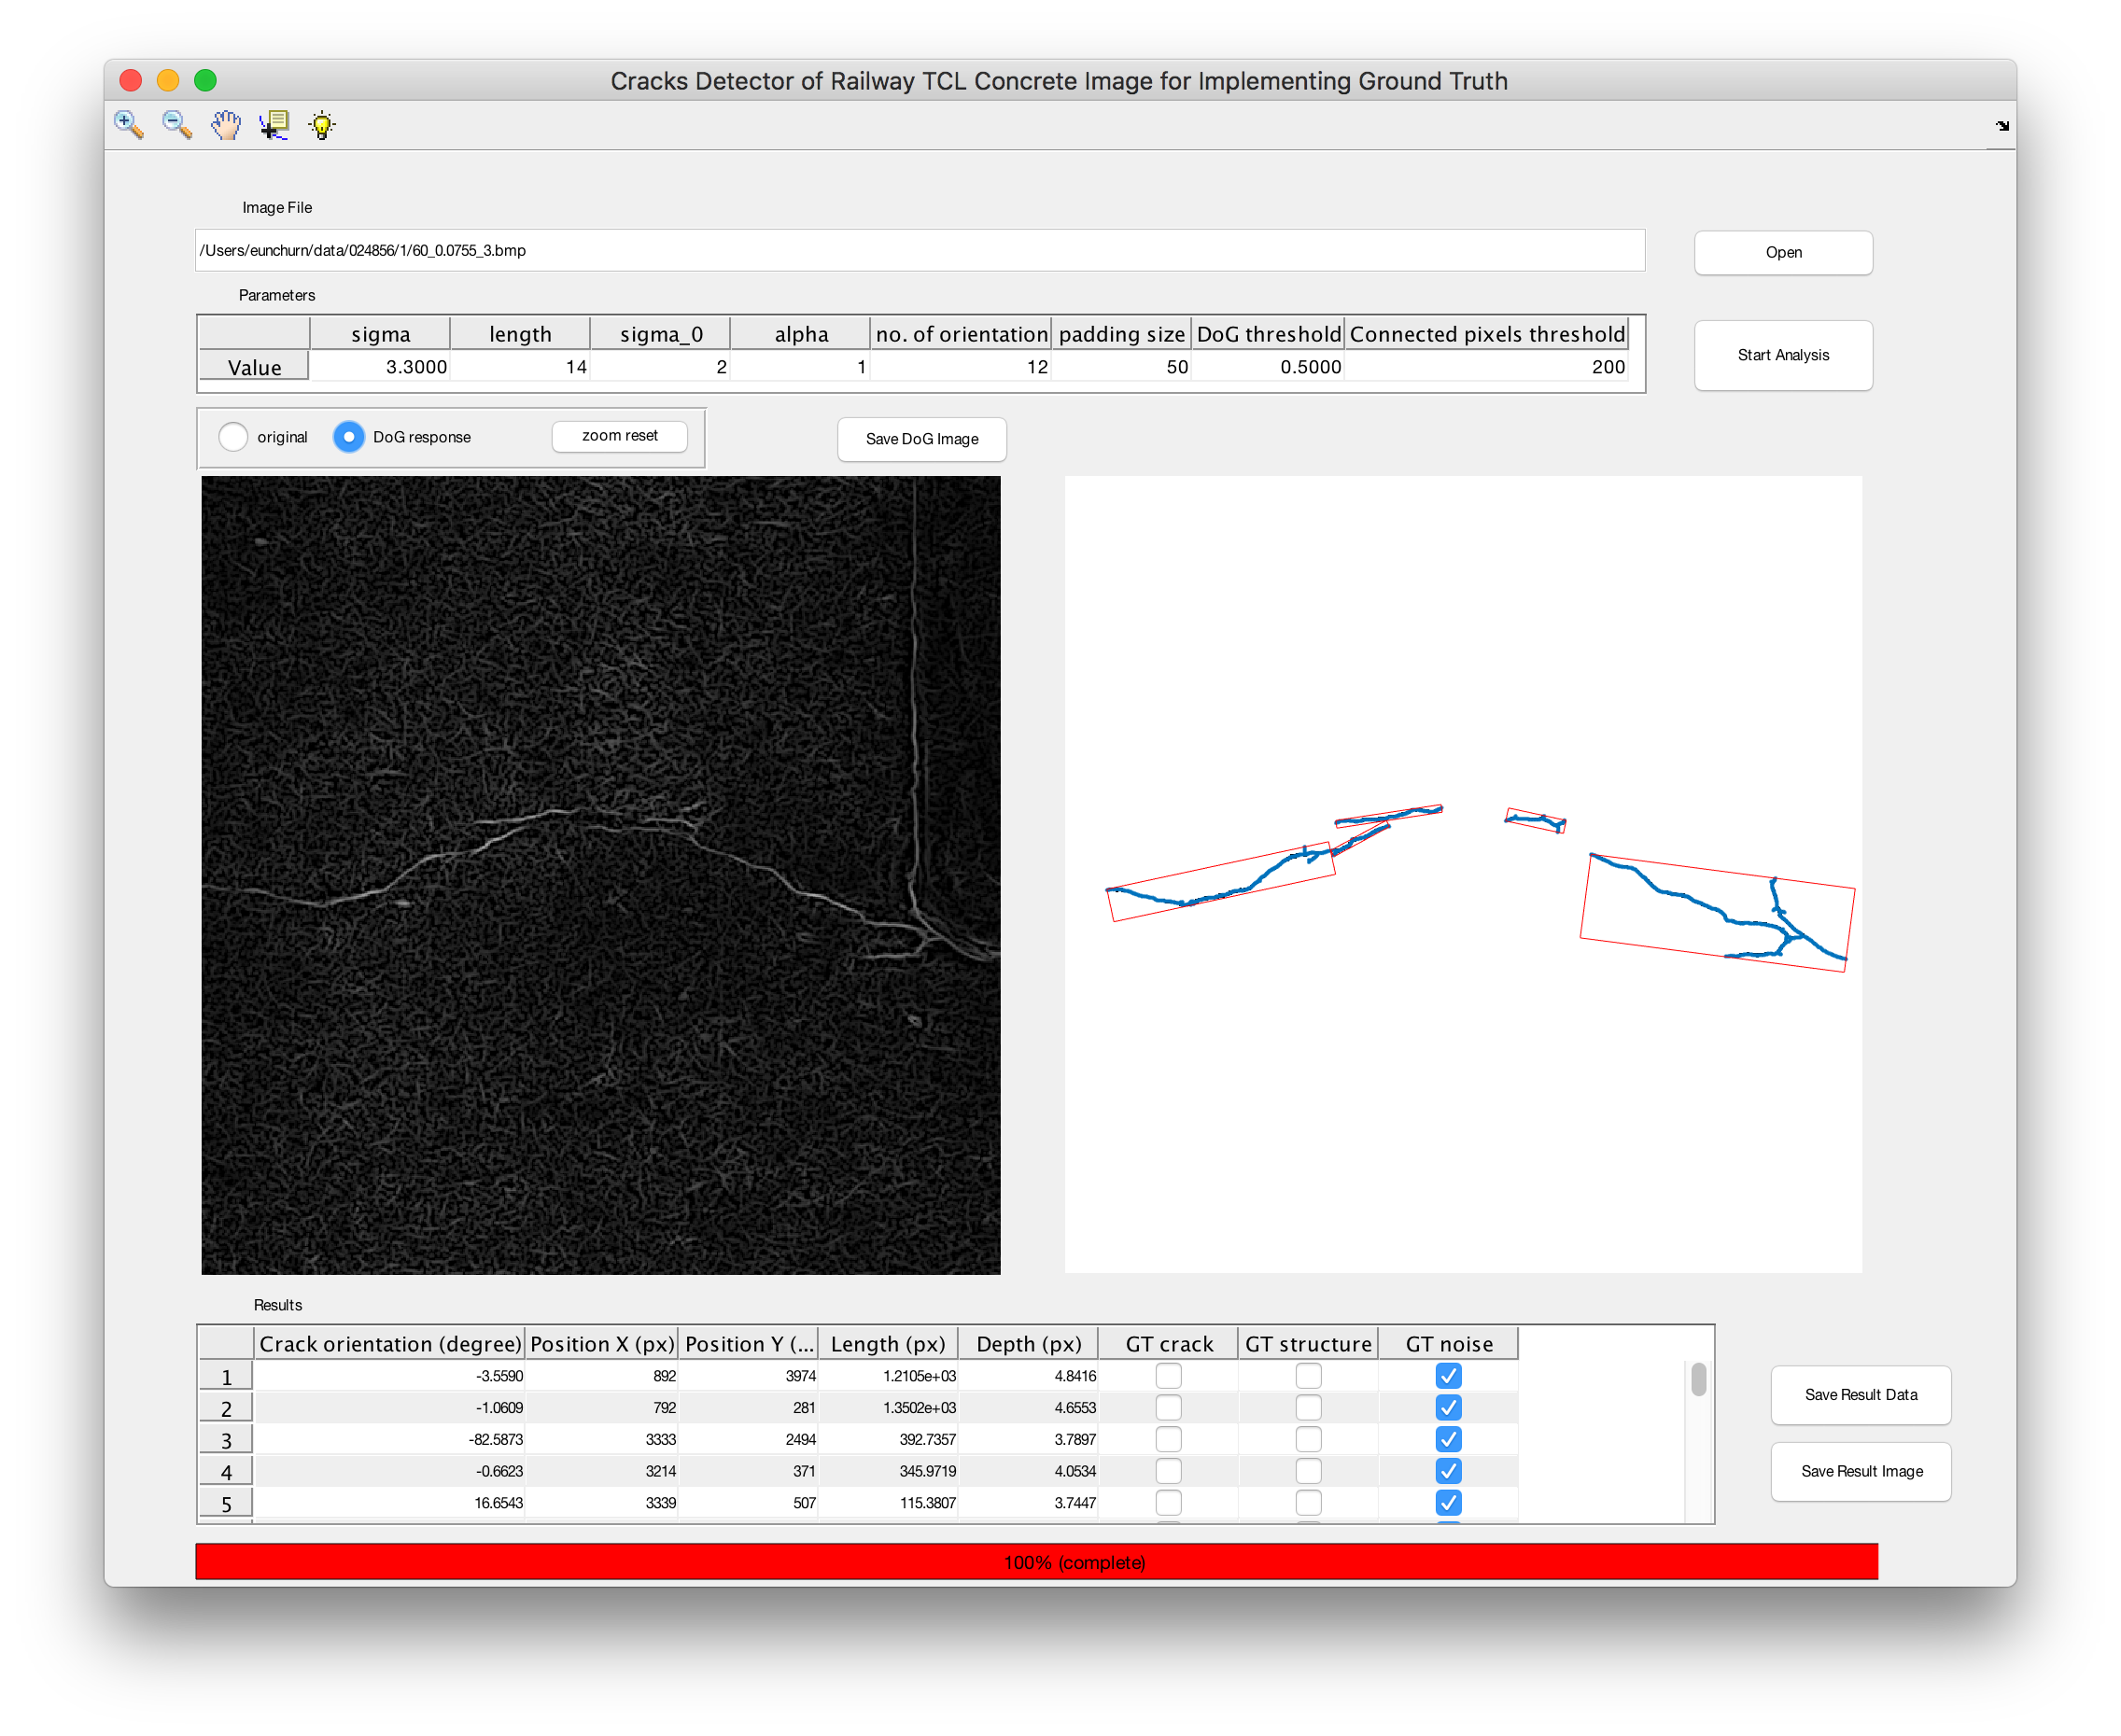
\includegraphics[width=0.5\textwidth]{images/zoomed_dog.png}
			\caption*{균열과 구조물 분리}
		}\qquad
		\parbox{0.5\textwidth}{
			\centering
			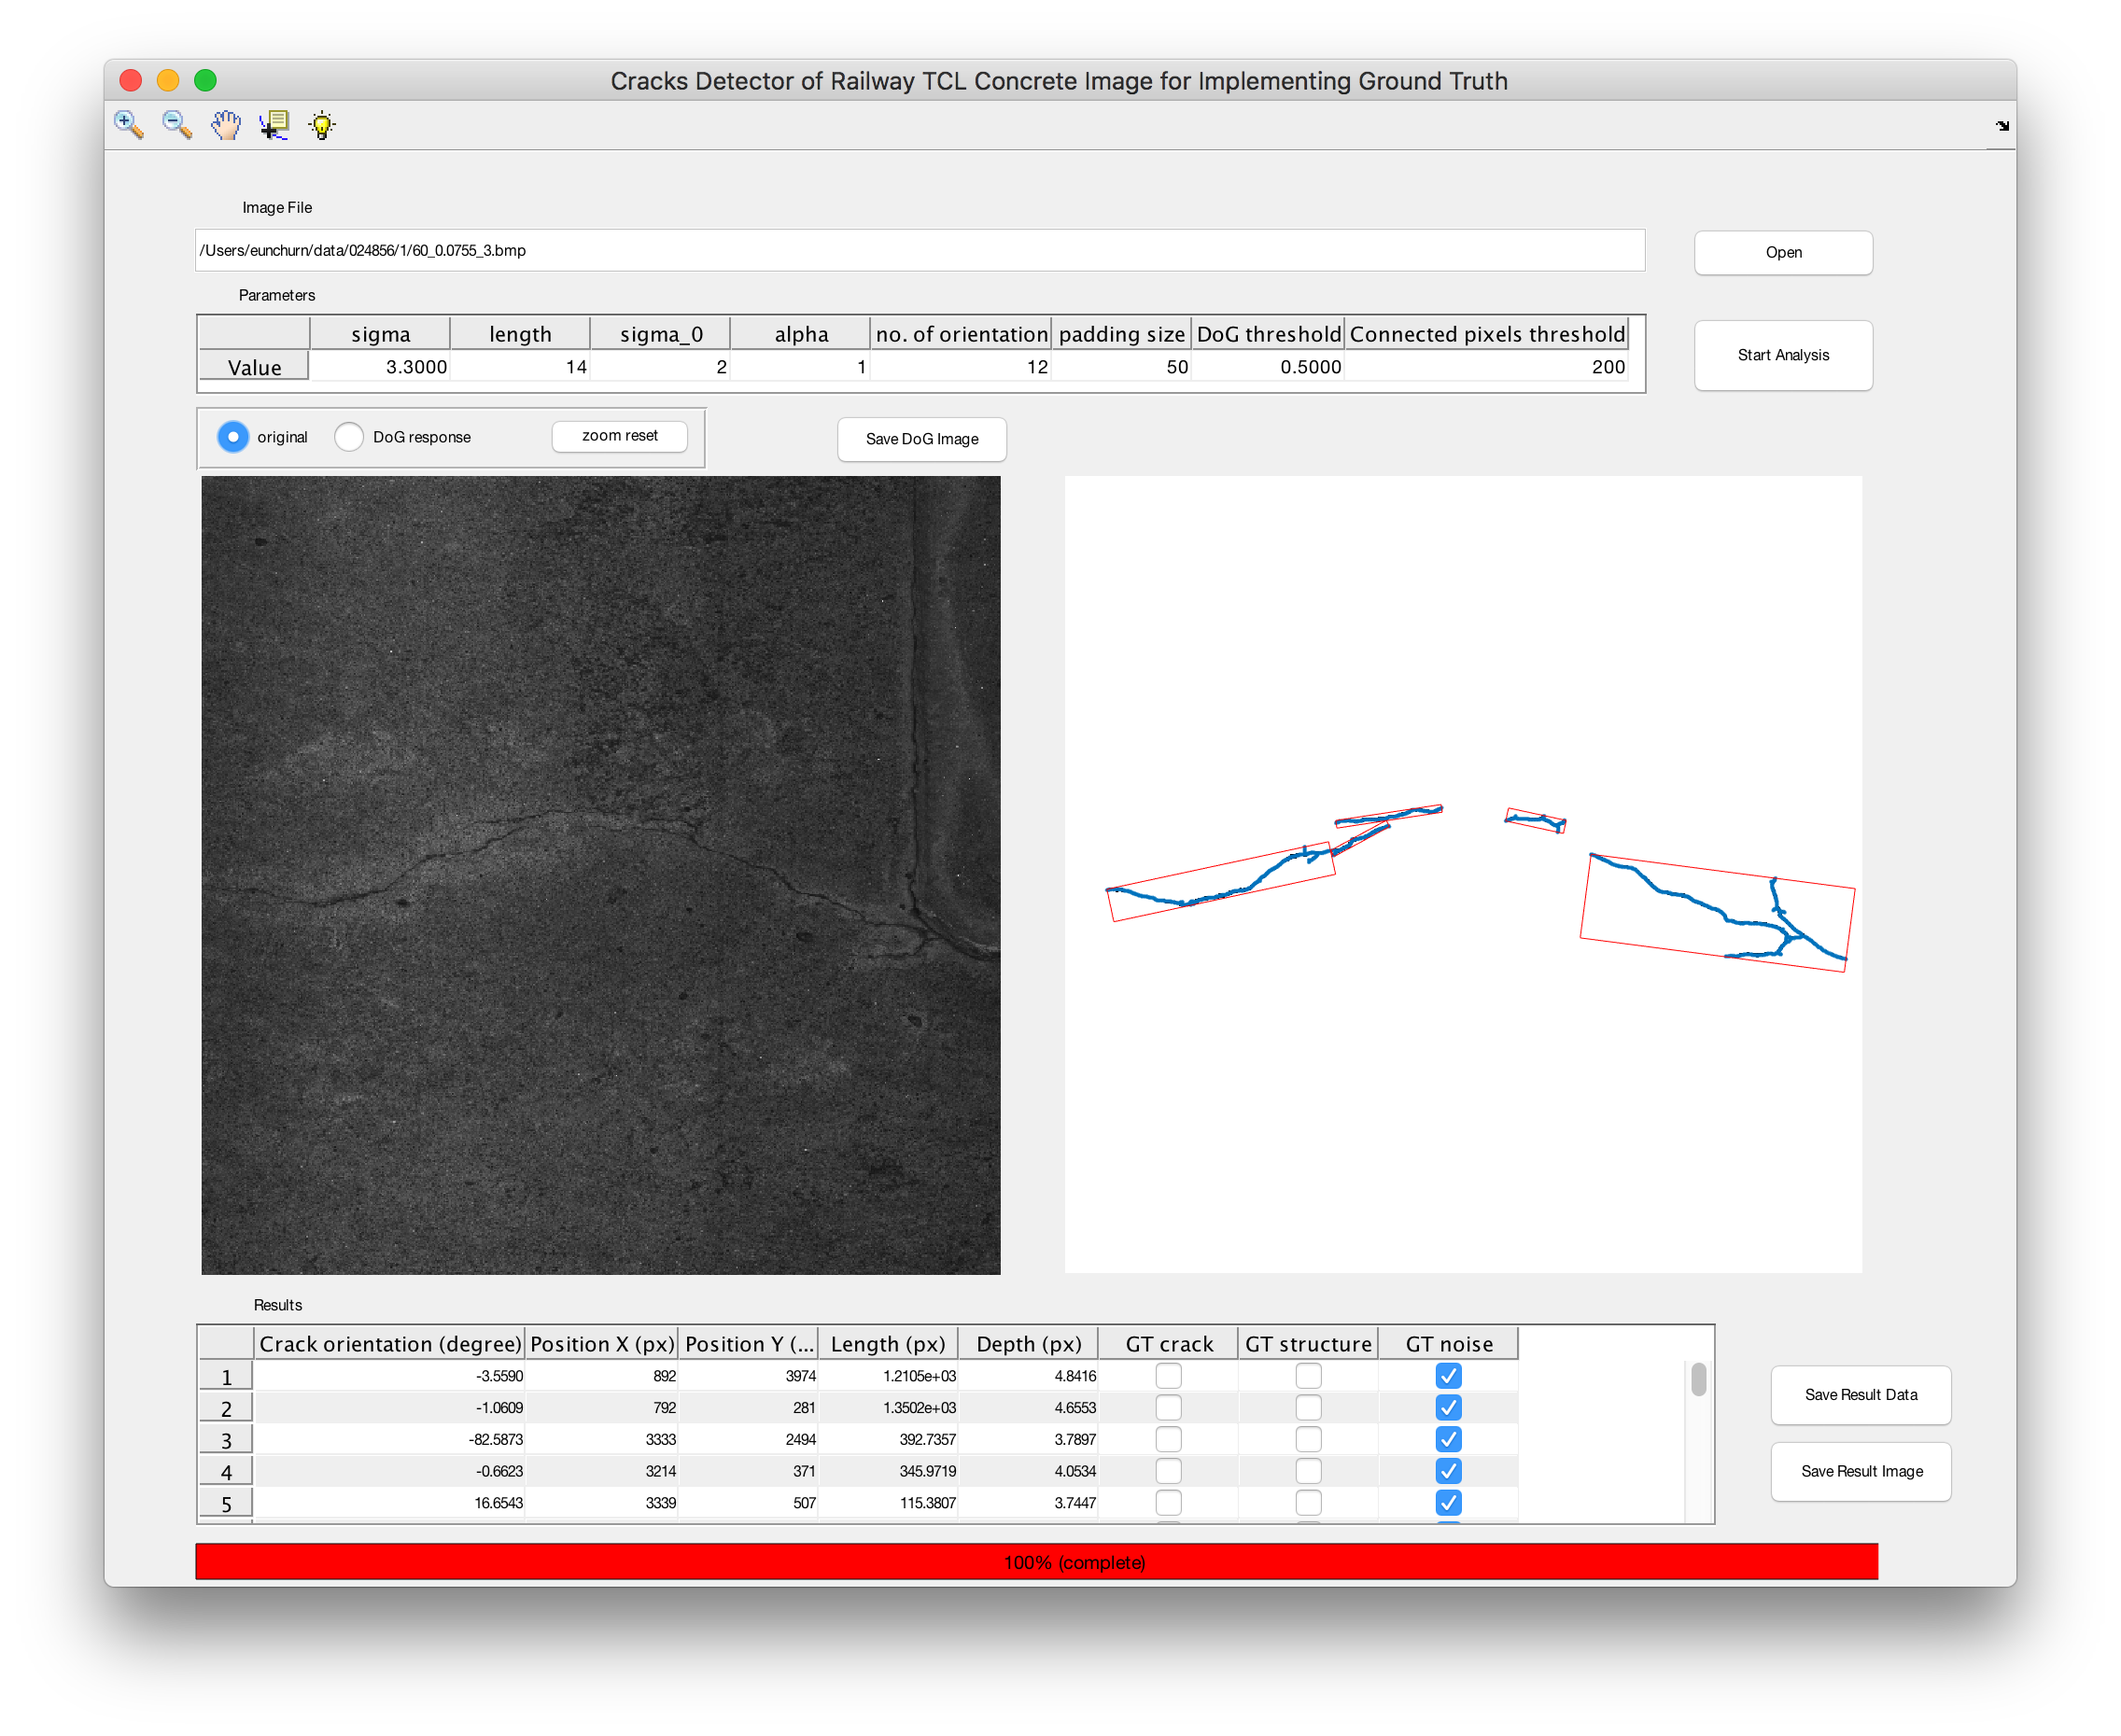
\includegraphics[width=0.5\textwidth]{images/zoomed.png}
			\caption*{균열 ground truth 지정}
		}\qquad
		\parbox{0.5\textwidth}{
			\centering
			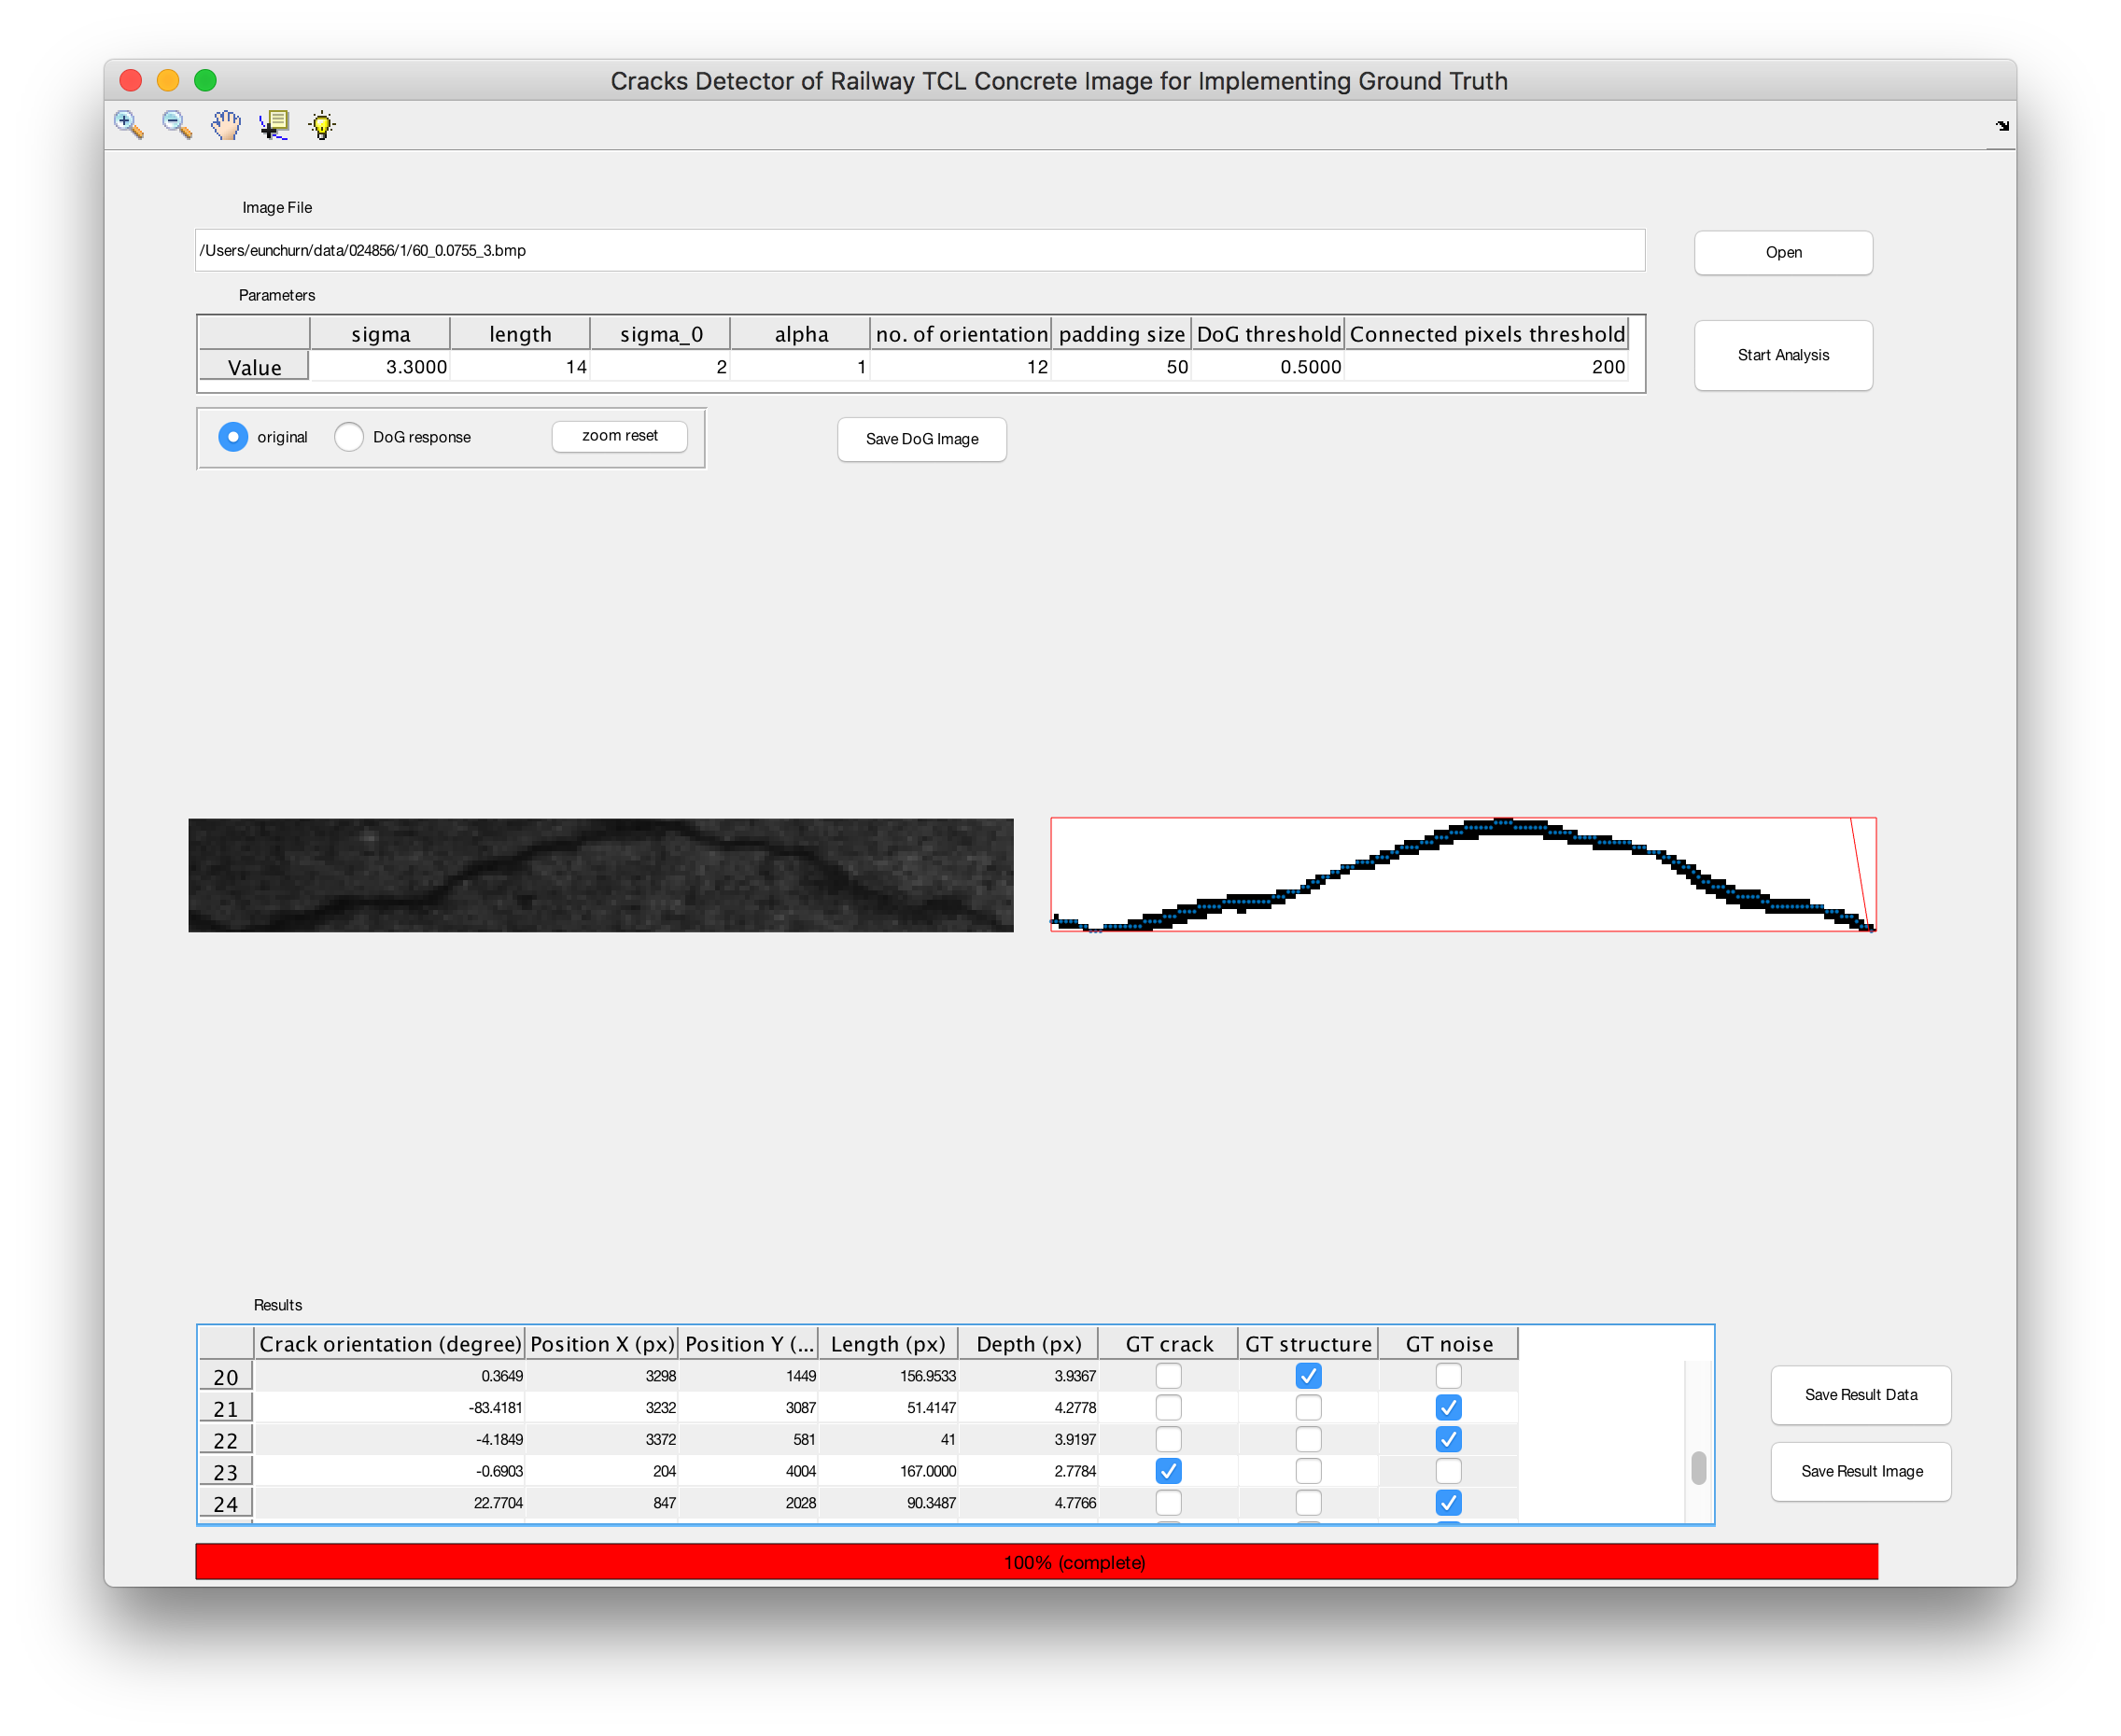
\includegraphics[width=0.5\textwidth]{images/crack06.png}
			\caption*{0.2mm 미세균열 검출}
		}
	\end{fullwidth}
\end{figure}

\divider

\cvevent{\printinfo{\faPlusSquare}{KTX 승객 검표지원 시스템 지능형 CCTV \& MTIT 연동}}{승화기술정책연구소(주) 개발참여: 100\%}{2016 -- 2017}{Seoul, Korea}

\label{korail}

\begin{itemize}[label=\emoji{satellite}]
	\item 소개: 컴퓨터 비젼(OpenCV) 및 이미지 프로세싱을 이용한 승객 착석유무 판단
	\item 참여 개발 내용
	      \begin{itemize}[label=\emoji{pushpin}]
		      \item 현장 CCTV를 통해 이미지 취득 후 컴퓨터 비젼 프로세싱
		      \item 개발 스택 및 프레임워크: C++ 기반 OpenCV, JavaScript(ES5), NodeJS, Express, EJS, Redis, MongoDB
		      \item KTX 1편성, ITX-청춘 1편성 현장 적용 완료
	      \end{itemize}
\end{itemize}

\begin{figure}[!ht]
	\begin{fullwidth}
		\parbox{0.5\textwidth}{
			\centering
			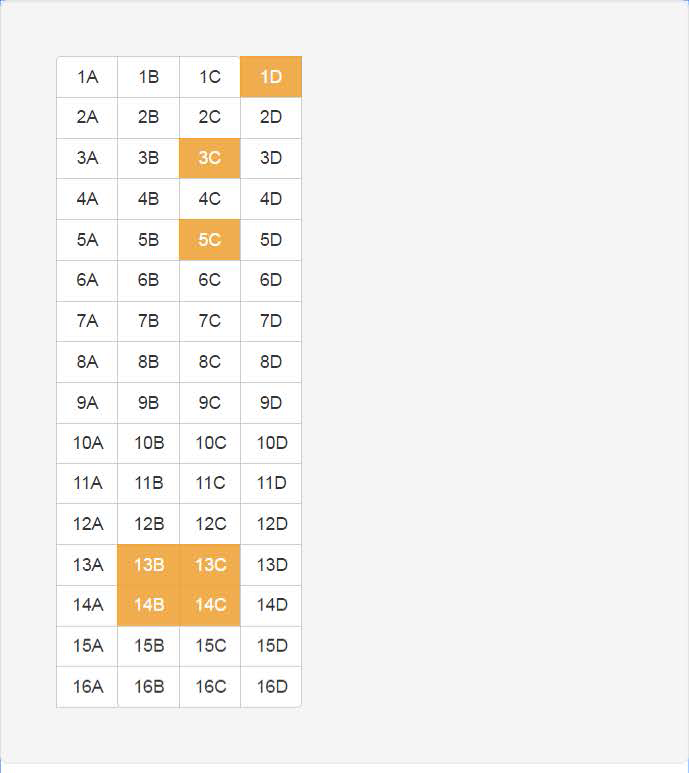
\includegraphics[width=0.5\textwidth]{images/korail_seat_01_01.png}
			\caption*{무임 승차자 검출}
		}\qquad
		\parbox{0.5\textwidth}{
			\centering
			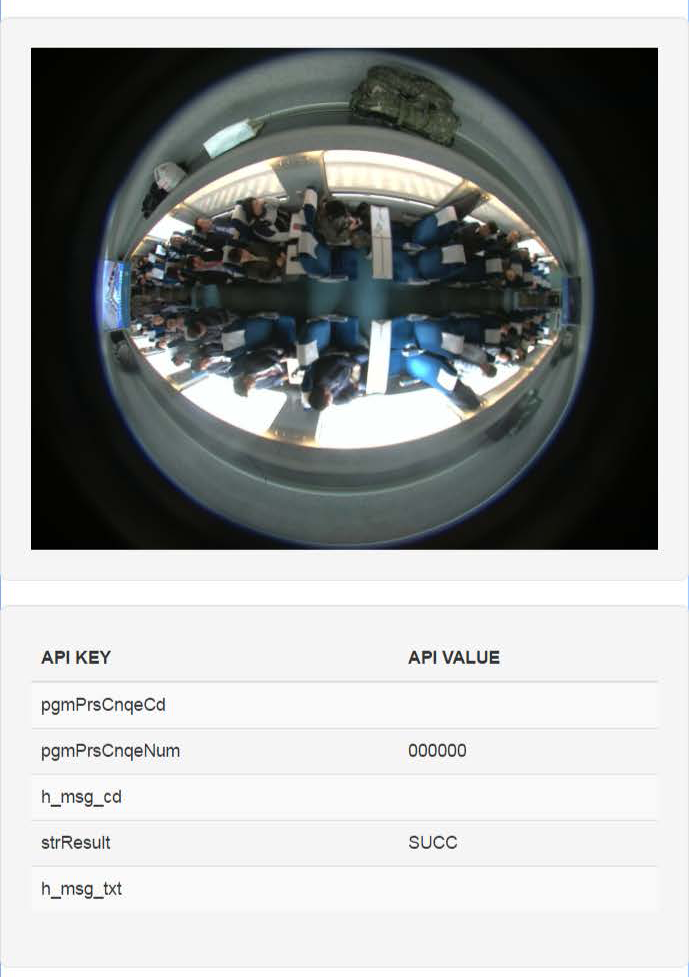
\includegraphics[width=0.5\textwidth]{images/korail_seat_01_02.png}
			\caption*{MTIT 발권 데이터 요청/응답}
		}\qquad
		\parbox{0.5\textwidth}{
			\centering
			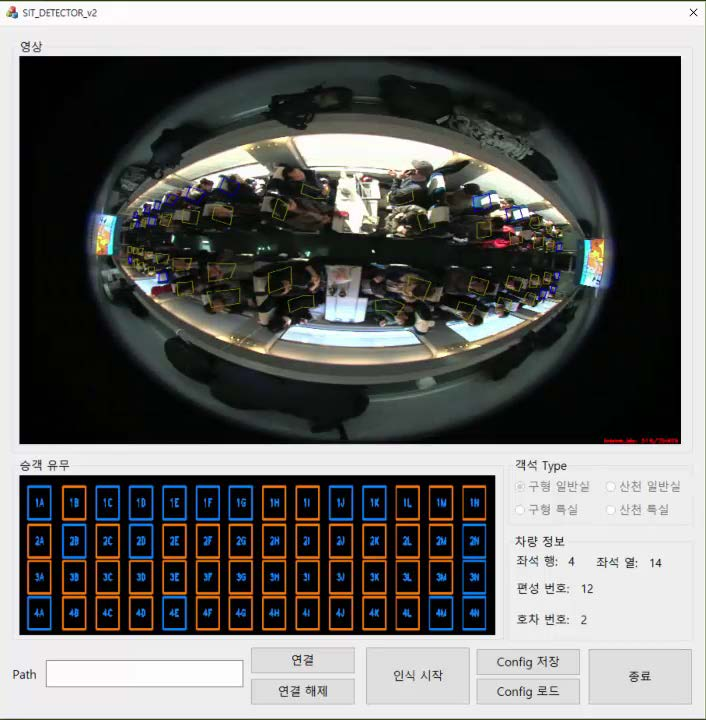
\includegraphics[width=0.5\textwidth]{images/korail_seat_02.jpg}
			\caption*{Raspberry Pi 탑재용 테스트 프로그램}
		}
	\end{fullwidth}
\end{figure}

\divider


\cvevent{\printinfo{\faPlusSquare}{철도 재해우려개소 지능형 CCTV 낙석감지 시스템}}{승화기술정책연구소(주) 개발참여: 95\%}{2016 -- 2017}{Seoul, Korea}

\begin{itemize}[label=\emoji{satellite}]
	\item
	      소개: 컴퓨터 비젼(OpenCV) 및 이미지 프로세싱을 이용한 낙석감지 알람
	\item 참여 개발 내용
	      \begin{itemize}[label=\emoji{pushpin}]
		      \item 현장 CCTV를 통해 이미지 취득 후 컴퓨터 비젼 프로세싱
		      \item 애플리케이션 개발: Raspberry Pi, NodeJS 애플리케이션(OpenCV, nodeJS, Redis, MongoDB 웹서버 및 UI가동)
		      \item 개발 스택 및 프레임워크
		            \begin{itemize}
			            \item C++ 기반 OpenCV
			            \item NVidia Jetson TX-1을 이용한 컴퓨터 비전 활용
			            \item JavaScript(ES5), NodeJS, Express, SocketIO 푸시 알림 웹서버 (Redis, MongoDB)
		            \end{itemize}
		      \item 현장 테스트베드 가동: 태백선 예미역
					\item 낙석 우려개소: 172여개소 적용
		      
	      \end{itemize}
	      \begin{figure}[!ht]
		      \begin{fullwidth}
			      \parbox{0.5\textwidth}{
				      \centering
				      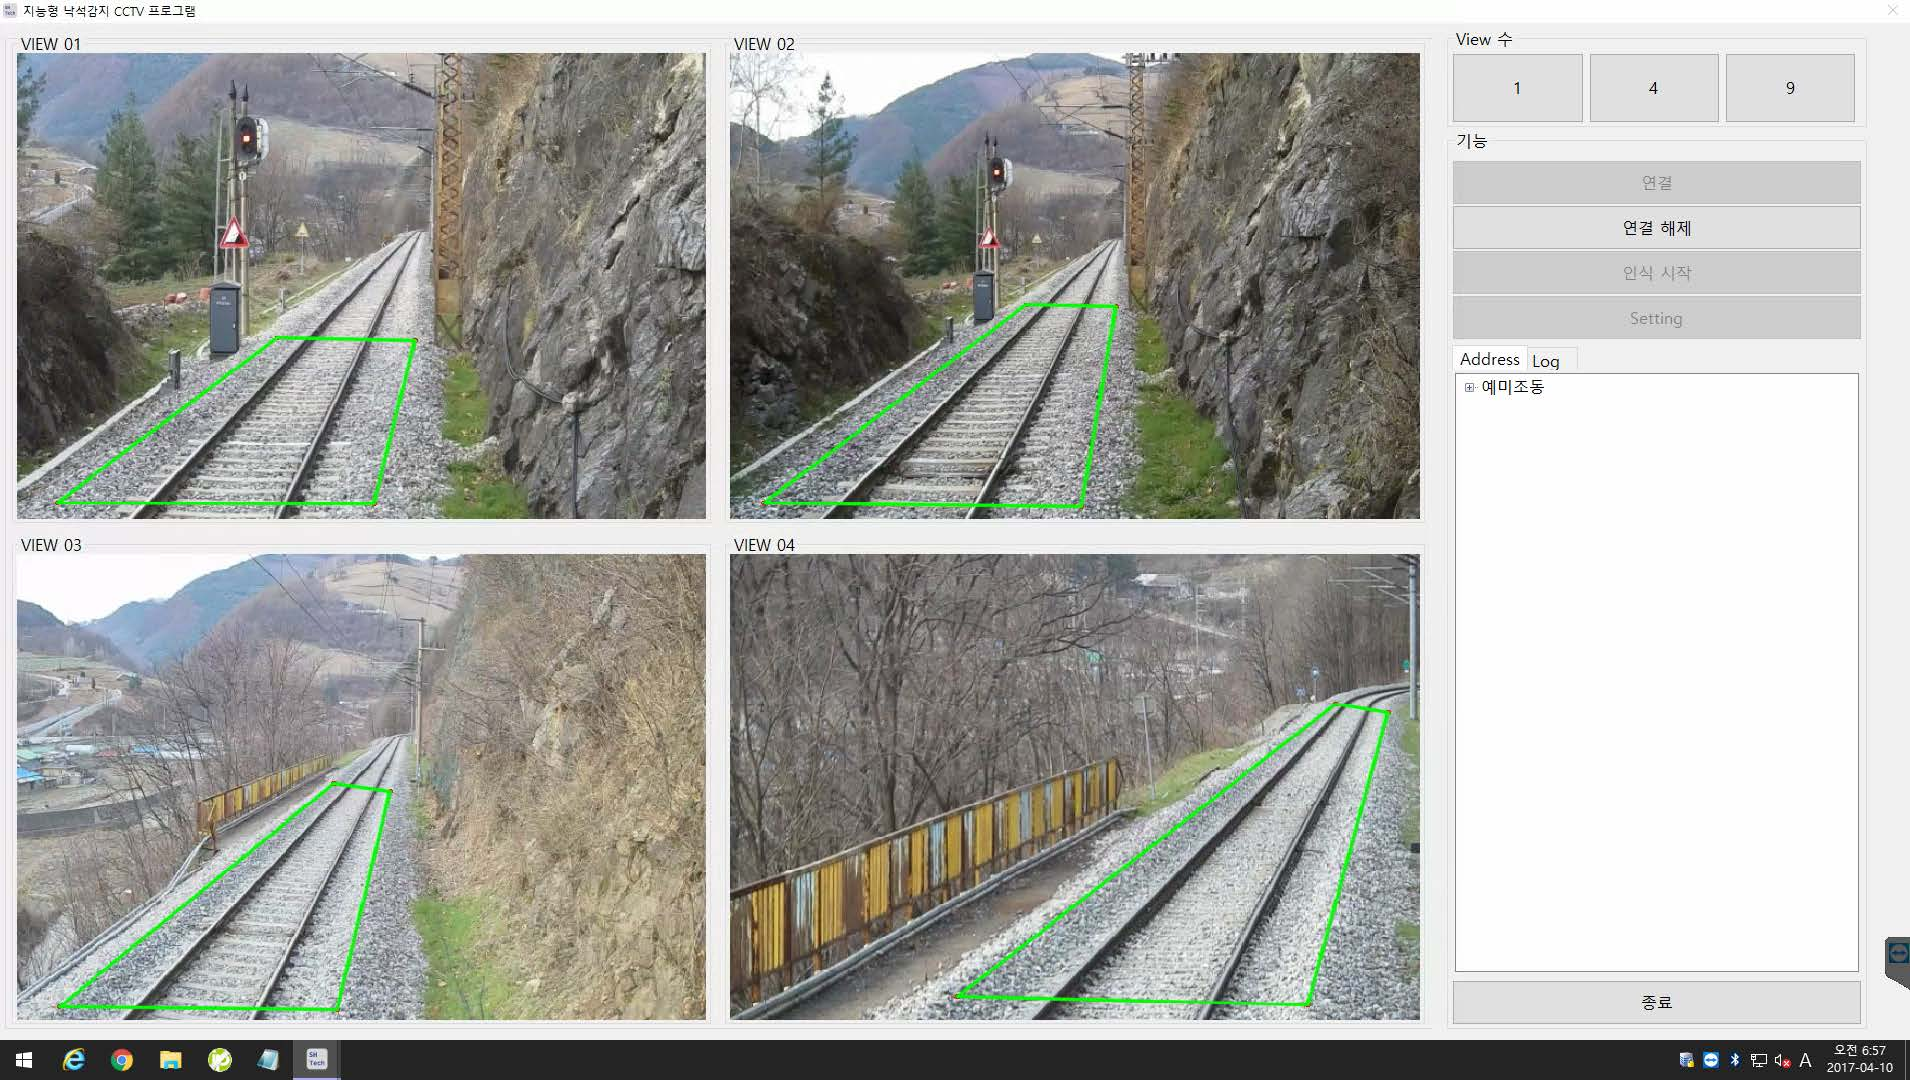
\includegraphics[width=0.5\textwidth]{images/korail_aod_01.jpg}
				      \caption*{OpenCV 애플리케이션}
			      }\qquad
			      \parbox{0.5\textwidth}{
				      \centering
				      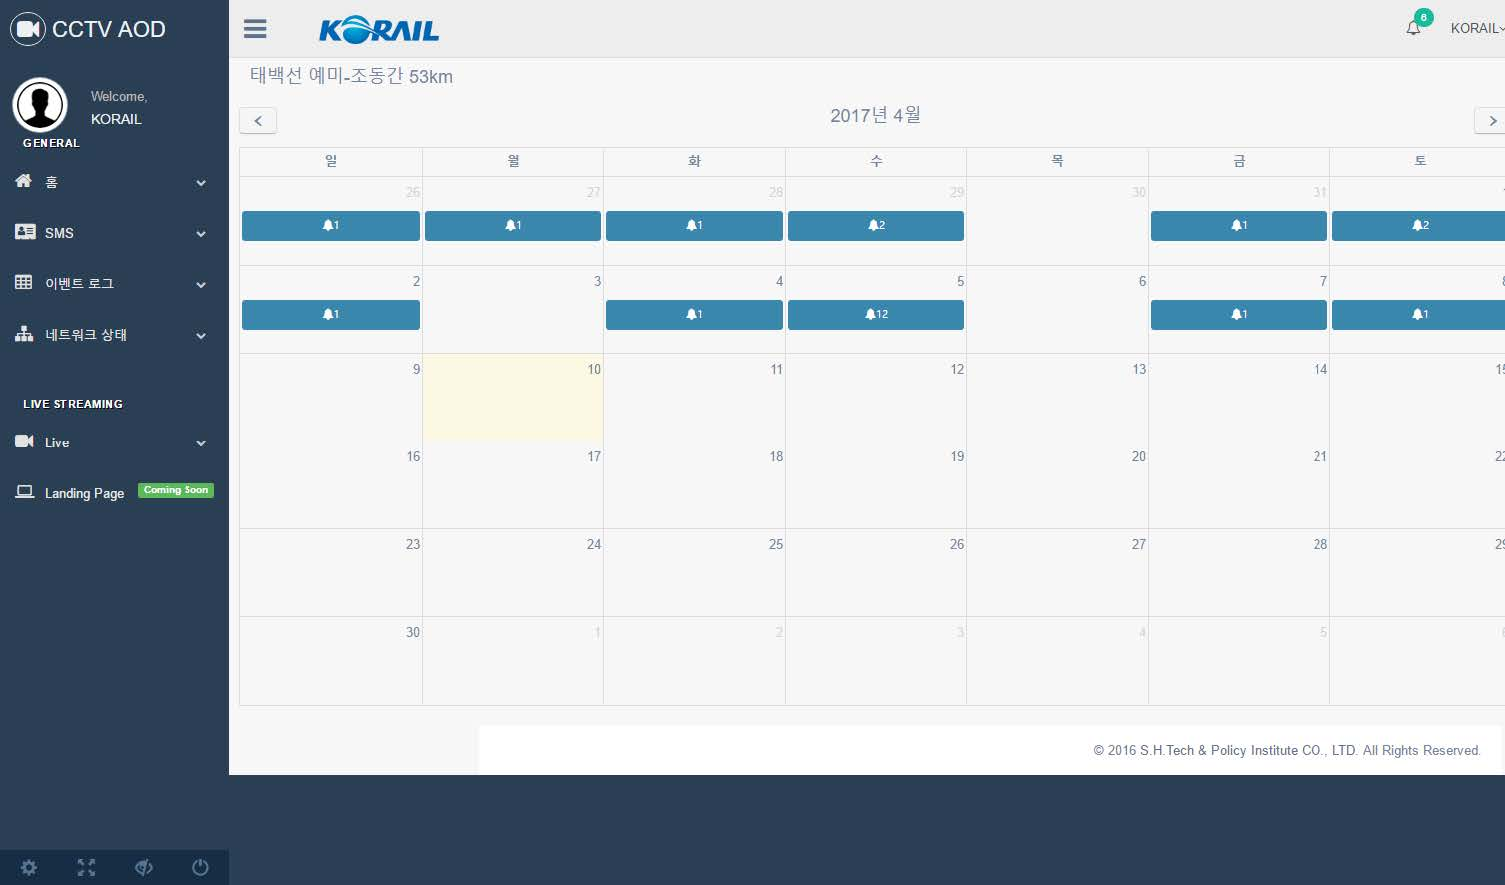
\includegraphics[width=0.5\textwidth]{images/korail_aod_02.jpg}
				      \caption*{이벤트 발생 기록}
			      }\qquad
			      \parbox{0.5\textwidth}{
				      \centering
				      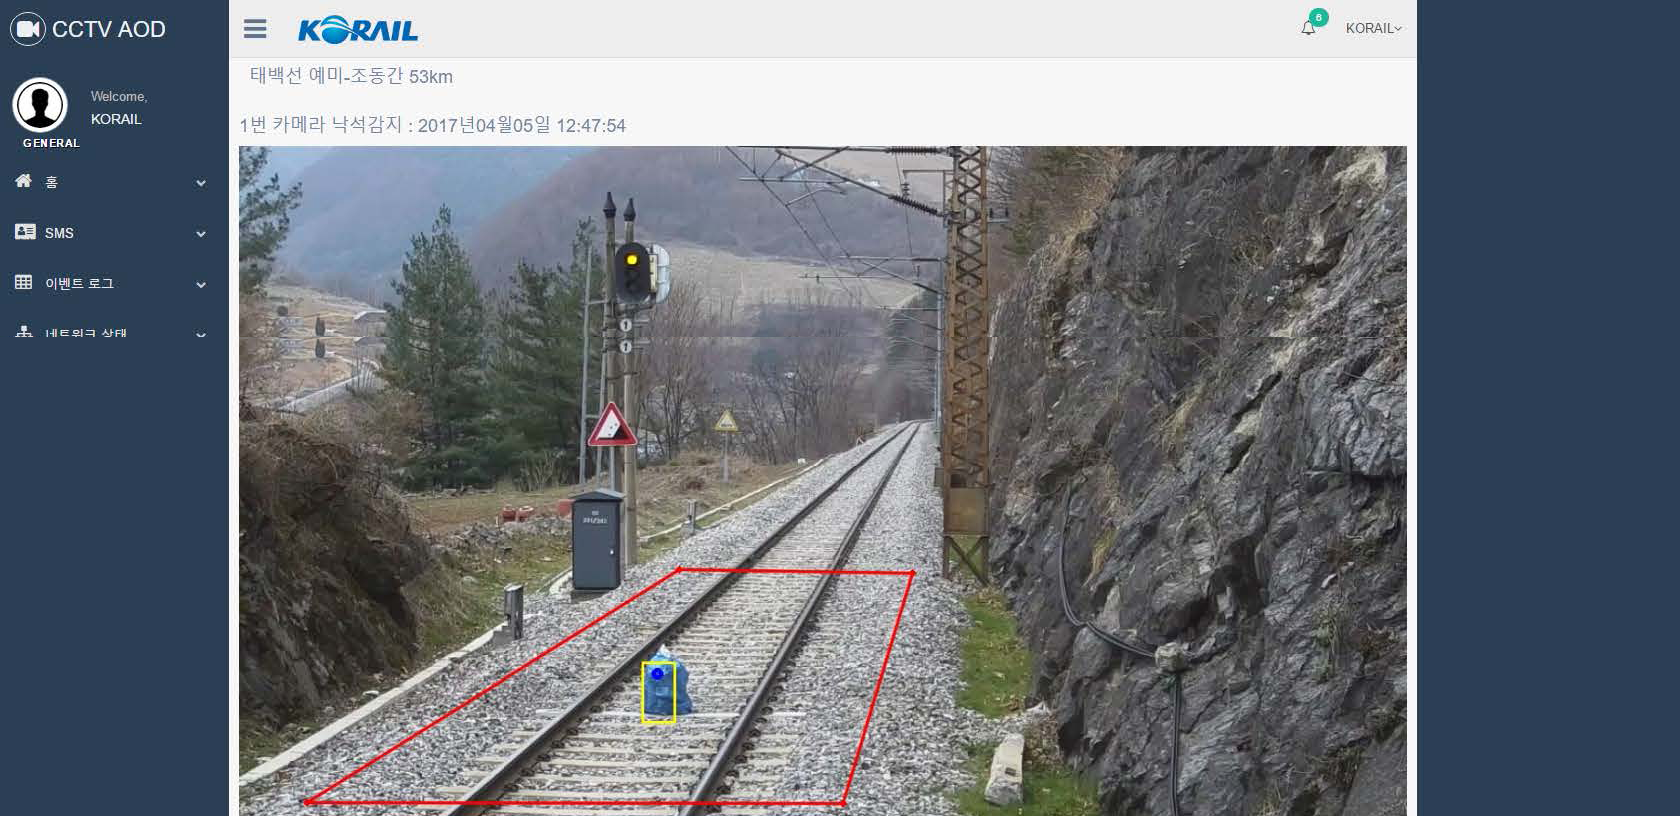
\includegraphics[width=0.5\textwidth]{images/korail_aod_03_01.png}
				      \caption*{이벤트 뷰 > SMS 메시지 전송}
			      }
		      \end{fullwidth}
	      \end{figure}
\end{itemize}

\divider

\cvevent{\printinfo{\faPlusSquare}{지하철 역사 초기 재난 대응 M2M 대피경로 안내 시스템}}{승화기술정책연구소(주) 개발참여: 80\%}{2015 -- 2017}{Seoul, Korea}

\label{m2m}

\begin{itemize}[label=\emoji{satellite}]
	\item 소개: 가스센서 노드로부터 데이터를 받아 화재 및 재난을 초기 인식하여 승객들에게 대피경로를 안내하는 시스템
	\item 참여 개발 내용:
	      \begin{itemize}[label=\emoji{pushpin}]
		      \item Libelium Waspmote기반 가스센서 펌웨어 개발
		      \item 가스센서 Calibration : MATLAB을 이용하여 기준값 측정 후 곡선적합
		      \item 게이트웨이 개발: Raspberry Pi \href{https://nodejs.org}{nodeJS} 애플리케이션(serial parsing, Redis, MongoDB, 웹서버 및 클라이언트 개발)

		            \begin{figure}[!ht]
			            \begin{fullwidth}
				            \centering
				            \parbox{0.8\textwidth}{
					            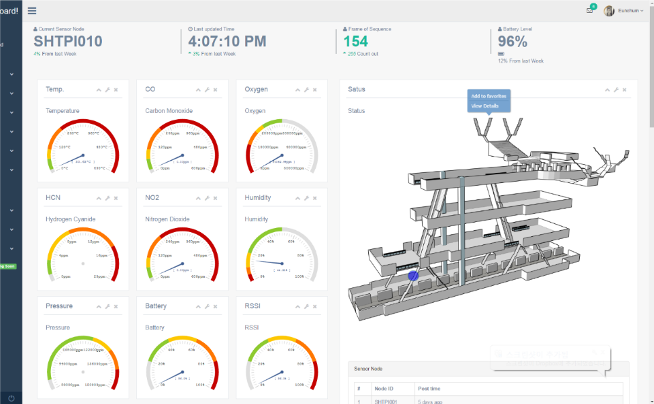
\includegraphics[width=0.8\textwidth]{images/m2m_01.png}
					            \caption*{실시간 센서 모니터링}
				            }\qquad
				            \parbox{0.8\textwidth}{
					            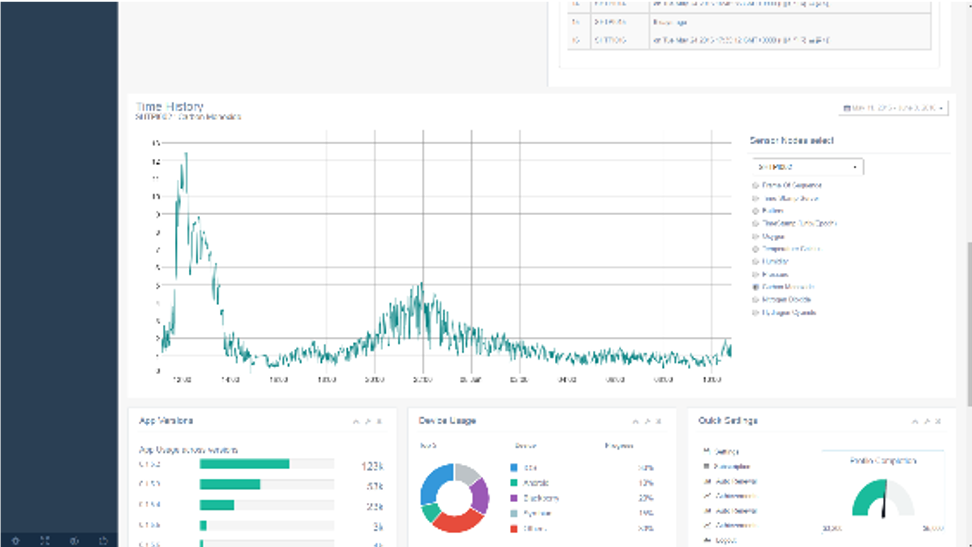
\includegraphics[width=0.8\textwidth]{images/m2m_02.png}
					            \caption*{센서 캘리브레이션, 데이터 조회}
				            }
			            \end{fullwidth}
		            \end{figure}
		      \item 센서노드 API 제작(Plug\&Sense): sleep time 스케쥴링
		      \item 화재 감지 및 화재 발생 위치 분석: 주요요소분석(principal component analysis, 각 센서데이터의 확률밀도함수와 이벤트간 주요요소분석), 확률변수시물레이션(Monte-Carlo 시물레이션)
		      \item Markov-chain 룰을 통해 상태예측 알고리즘 개발
		      \item 대피경로 안내 시스템 개발(역무원용/승객 알림용)
		            \begin{figure}[ht!]
			            \begin{fullwidth}
				            \centering
				            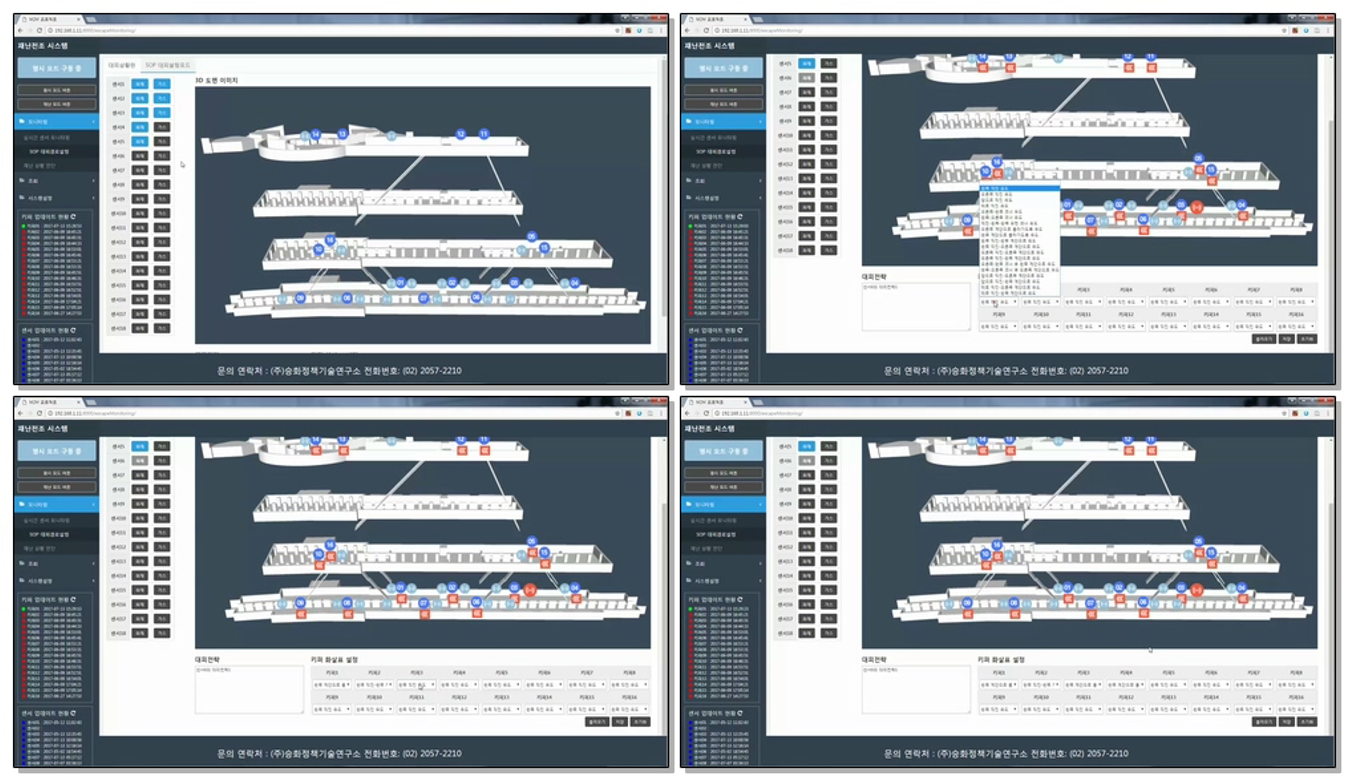
\includegraphics[width=1.2\textwidth]{images/m2m_03.png}
				            \caption*{대피경로 안내 시나리오 설정}
			            \end{fullwidth}
		            \end{figure}
		            \begin{figure}[ht!]
			            \begin{fullwidth}
				            \centering
				            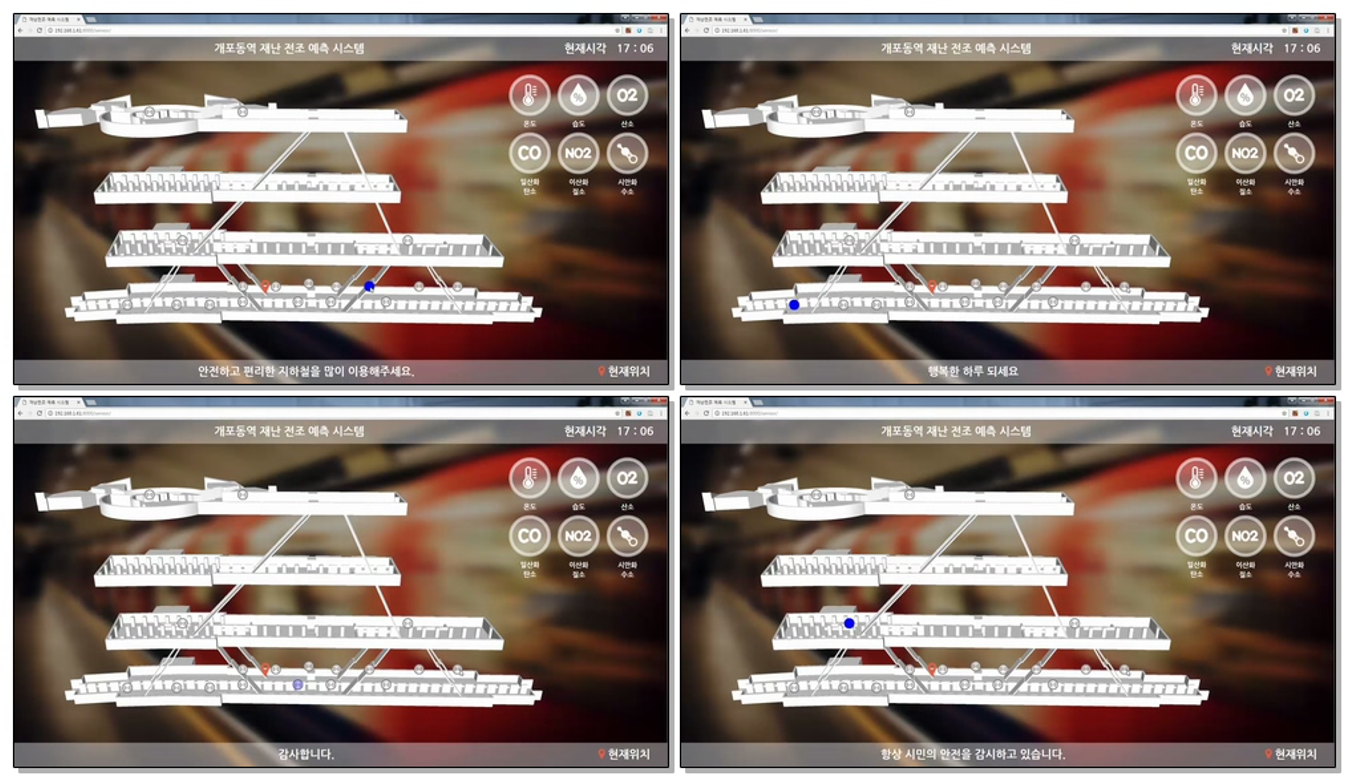
\includegraphics[width=1.2\textwidth]{images/m2m_04.png}
				            \caption*{승객용 재난 발생 위치 알림}
			            \end{fullwidth}
		            \end{figure}
		            \begin{figure}[ht!]
			            \begin{fullwidth}
				            \centering
				            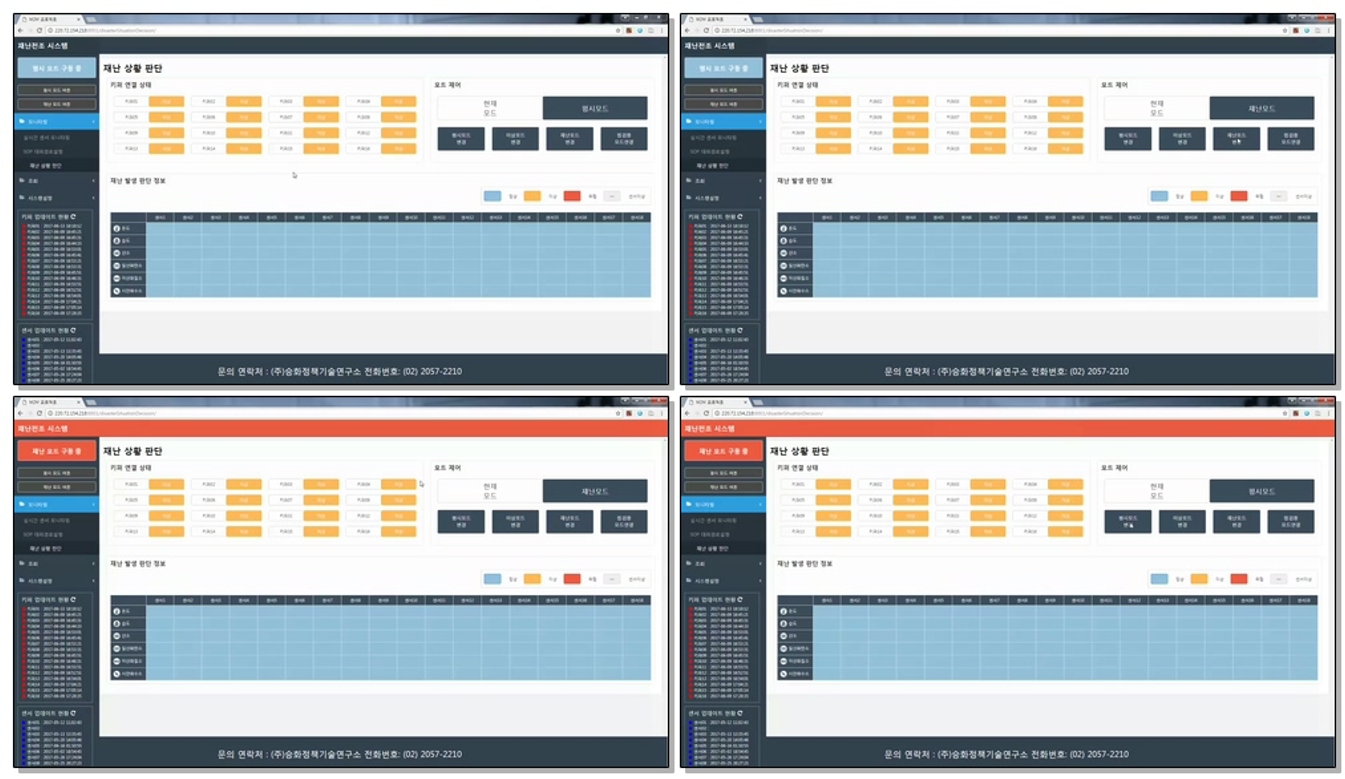
\includegraphics[width=1.2\textwidth]{images/m2m_05.png}
				            \caption*{센서 Matrix Rule set 지정}
			            \end{fullwidth}
		            \end{figure}
		      \item 적용된 기술:
		            \begin{itemize}
			            \item \href{https://en.wikipedia.org/wiki/Machine_to_machine}{M2M}
			            \item \href{https://lora-alliance.org/}{LoRa} 802.11ah SX1274 916MHz
			            \item \href{https://en.wikipedia.org/wiki/Principal_component_analysis}{Principal component analysis}
			            \item \href{https://en.wikipedia.org/wiki/Monte_Carlo_method}{Monte Carlo method}
			            \item \href{https://en.wikipedia.org/wiki/Markov_chain}{Markov chain}
		            \end{itemize}
		      \item 개발 스택 및 프레임워크
		            \begin{itemize}
			            \item 적합성 데이터 분석 및 센서 캘리브레이션: Mathworks MATLAB
			            \item 센서 관리 웹어드민: JavaScript(ES5), NodeJS, Express, React, Webpack
			            \item 센서 데이터 송신 펌웨어: C (Libelium SDK)
			            \item 센서 특징 정보 추출: Python
			            \item 대피경로 안내 시스템: Django
		            \end{itemize}
		      \item 참여한 현장: 대공원역 / 개포동역
	      \end{itemize}
\end{itemize}
